\documentclass{beamer}
\usepackage{graphicx}
\usetheme{Boadilla}

\begin{document}

\title[ICER 2013]{An Open System for\\
Managing Short Programming Exercises}
\author[Papancea et.\ al.]{Andrei Papancea\textsuperscript{*}, Jaime Spacco\textsuperscript{*}, and David Hovemeyer\textsuperscript{$\dagger$}}
\institute[Knox, YCP]{
\begin{minipage}[t]{1.1in}
\begin{center}
{{\ }\\
\textsuperscript{*}Knox College}
\vskip .1in

\includegraphics[height=.8in]{images/KnoxLogo}
\end{center}
\end{minipage}
\begin{minipage}[t]{1.1in}
\begin{center}
{\textsuperscript{$\dagger$}York College\\
of Pennsylvania}
\vskip .1in

\includegraphics[height=.8in]{images/YCPLogo}
\end{center}
\end{minipage}
}
\date[August, 2013]{ICER\\
August 12, 2013}

\begin{frame}[plain]
  \titlepage
\end{frame}

%%%%%%%%%%%%%%%%%%%%%%%%% Outline %%%%%%%%%%%%%%%%%%%%%%%%%%%
%\begin{frame}{Outline}
%
%\begin{itemize}
%  \item Background
%  \item Description of CloudCoder
%  \item Preliminary Experiences
%  \item Questions
%\end{itemize}
%
%\end{frame}

%%%%%%%%%%%%%%%%%%%%%%%% Background %%%%%%%%%%%%%%%%%%%%%%%%%%%
\begin{frame}{Background}

\begin{itemize}
  \item Many students struggle in introductory programming courses
  \item Mastery of basic concepts and techniques is essential for success
  \item Short programming exercises ({\` a} la CodingBat):
  \begin{itemize}
    \item Web-based UI
    \item Students write or complete a short (5-15 line) function or program
    \item Correctness is judged with a series of test cases
    \item Student receives immediate feedback
  \end{itemize}
  \item Useful for:
  \begin{itemize}
    \item Skills development
    \item Self-tests to accompany reading
    \item Extra practice
  \end{itemize}
\end{itemize}

\end{frame}

%%%%%%%%%%%%%%%%%%%%%%%% Why another system? %%%%%%%%%%%%%%%%%%%%%%%%%%%
\begin{frame}{Why another system?}

\begin{itemize}
  \item There are lots of programming exercise systems already:
  \begin{itemize}
    \item Free: CodingBat, PracticeIt!, Codecademy
    \item Commercial: CodeLab (TuringsCraft), MyProgrammingLab (Pearson)
    \item {\em Do we really need another one?}
  \end{itemize}
  \item We did not know of one that
  \begin{itemize}
    \item Encouraged users to create and share {\bf freely-redistributable} exercises
    \item Supported a range of languages (including C/C++)
    \item Was open source
    \item Collected rich data about how students work
  \end{itemize}
  \item We created a new system, called CloudCoder, to fill this niche
    \begin{itemize}
    \item \url{http://cloudcoder.org}
    \end{itemize}
\end{itemize}

\end{frame}

%%%%%%%%%%%%%%%%%%%%%%%% CloudCoder %%%%%%%%%%%%%%%%%%%%%%%%%%%
\begin{frame}{CloudCoder}

\begin{itemize}
  \item Open source (AGPL v3)
  \item Supports Java, Python, Ruby, and C/C++
  \item Repository of freely-redistributable (CC-BY-SA) exercises:
        \url{https://cloudcoder.org/repo}
    \begin{itemize}
    \item We encourage users to contribute, but do not require them to
    \end{itemize}
  \item Web-based user interface
    \begin{itemize}
    \item 100\% HTML/CSS/JavaScript, no plugin required
    \end{itemize}
  \item Collects fine-grained edit sequence of each student's work
\end{itemize}

\end{frame}

%%%%%%%%%%%%%%%%%%%%%%%% CloudCoder screenshot %%%%%%%%%%%%%%%%%%%%%%%%%%%
\begin{frame}{CloudCoder screenshot}

\begin{center}
\vskip -.15in
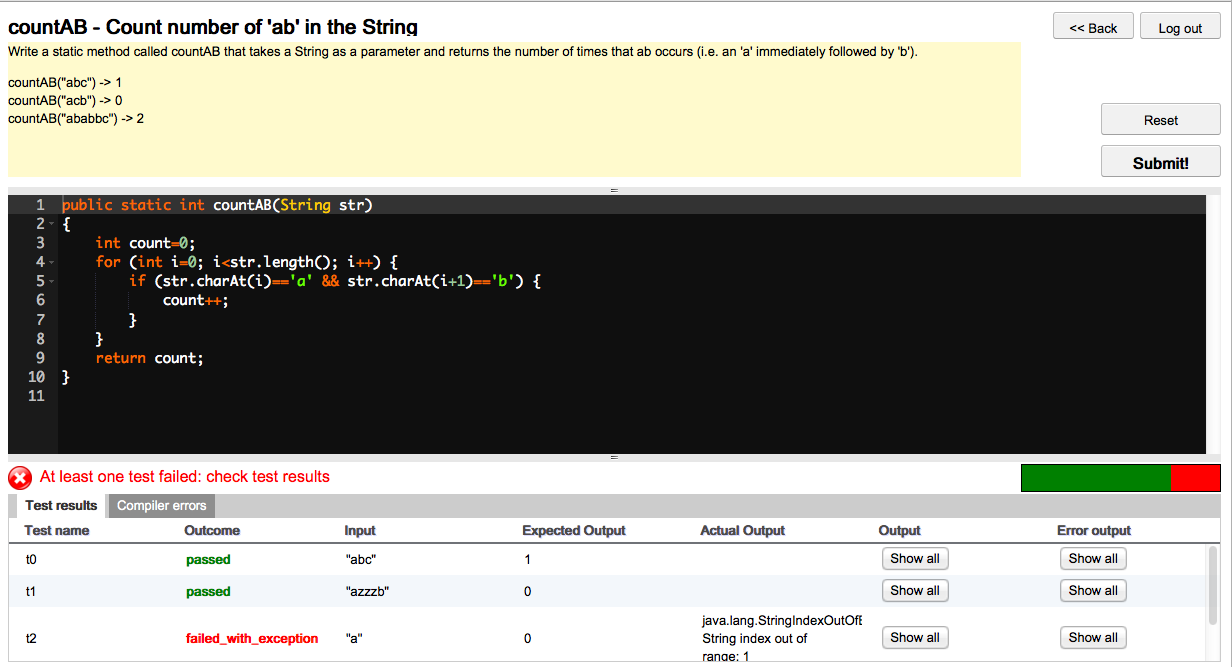
\includegraphics[width=4.5in]{images/screenshot5}
\end{center}

\end{frame}

%%%%%%%%%%%%%%%%%%%%%%%% Freedom matters %%%%%%%%%%%%%%%%%%%%%%%%%%%
\begin{frame}{Freedom matters}

\begin{itemize}
  %\item The impact of a pedagogical technique or curriculum resource
  %      depends on how many students can access it
  \item Goal: make programming exercises available to {\bf anyone} at {\bf any time} for {\bf any purpose}
  \begin{itemize}
    \item No payment
    \item No restrictive licenses
    \item No central control
  \end{itemize}
  \item Exercises can be used in many contexts:
  \begin{itemize}
    \item Our need: assign exercises in the context of a course
    \item In-class exercises to support peer instruction
          (PCRS, Zingaro et.\ al., SIGCSE 2013)
      %\begin{itemize}
      %\item Summer 2013: PCRS can import exercises from the CloudCoder exercise repository!
      %\end{itemize}
    \item Codecademy-style self-learning?
  \end{itemize}
\end{itemize}

\end{frame}

%%%%%%%%%%%%%%%%%%%%%%%%% Email #1 %%%%%%%%%%%%%%%%%%%%%%%%%%%
%\begin{frame}{Email \#1}
%
%\begin{center}
%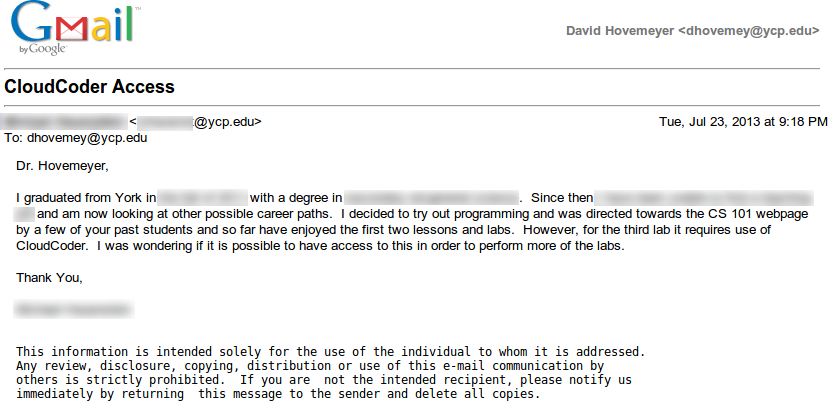
\includegraphics[width=4.5in]{images/email1}
%\end{center}
%
%[I (DH) created an account and replied with the username and password.]
%
%\end{frame}
%
%%%%%%%%%%%%%%%%%%%%%%%%% Email #2 %%%%%%%%%%%%%%%%%%%%%%%%%%%
%\begin{frame}{Email \#2}
%
%\begin{center}
%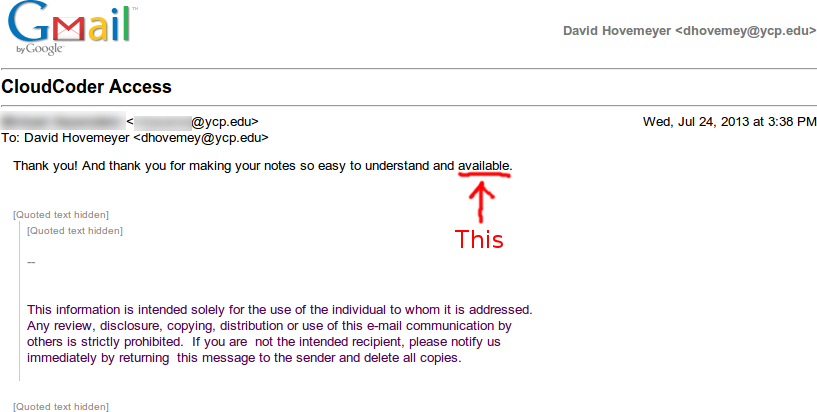
\includegraphics[width=4.5in]{images/email2}
%\end{center}
%
%\end{frame}

%%%%%%%%%%%%%%%%%%%%%%%% CloudCoder screenshot %%%%%%%%%%%%%%%%%%%%%%%%%%%
\begin{frame}{Hosting CloudCoder}

\begin{itemize}
  \item Requires two Linux servers to host (one network-facing)
    \begin{itemize}
    \item Relatively easy to install
    \item Known to work: 60+ concurrent users with modest hardware
    \item Load testing: 700+ concurrent users
          on moderate server hardware
      \begin{itemize}
      \item Compiling and testing submissions can require significant
            CPU resources, but are easy to scale up by adding more
            build servers
      \end{itemize}
    \item Cost to host per course-semester: perhaps \$1-\$3 per student
          (e.g., using Amazon EC2)
    \end{itemize}
  \item {\bf We can host CloudCoder for your course!}
    \begin{itemize}
    \item We have a grant from Amazon to cover hosting costs for
          a small number of institutions/courses
    \item {\bf Talk to us if you are interested!}
    \end{itemize}
\end{itemize}

\end{frame}

%%%%%%%%%%%%%%%%%%%%%%%% Experiences %%%%%%%%%%%%%%%%%%%%%%%%%%%
\begin{frame}{Experiences}

\begin{itemize}
\item Pilot studies:
  \begin{itemize}
  \item Canisius College: 30 students, CS1, C++
  \item York College: 122 students, CS1, C
  \item Knox College: 23 students, CS1, Java
  \item U.\ of Auckland: 30 students, CS1, C
  \end{itemize}
\item Experiences:
  \begin{itemize}
  \item The software works, students seem to like it
  \item Writing exercises from scratch is hard!
  \item Repository has 100+ exercises, but not much reuse has occurred yet
  \end{itemize}
\item Can we scale it to larger courses?
  \begin{itemize}
\item September 2013: U.\ of Auckland: 700 students, CS1, C
  \end{itemize}
\end{itemize}

\end{frame}

%%%%%%%%%%%%%%%%%%%%%%%% Questions %%%%%%%%%%%%%%%%%%%%%%%%%%%

\begin{frame}{Questions}

\begin{itemize}
\item Are short exercises useful?
  \begin{itemize}
  \item Do you use short exercises in your courses currently?
    \begin{itemize}
    \item If so, how?
    \item If not, would you be interested in starting to use them?
    \end{itemize}
  \item What experiments should we do to measure effect on outcomes?
  \end{itemize}
\item How to incorporate short exercises into a course most effectively?
  \begin{itemize}
  \item How do we know what exercises should be assigned?
  \item In what order should the exercises be assigned?
  \item What mix of short exercises vs.\ larger assignments?
  \item How to motivate students to attempt exercises?
    \begin{itemize}
    \item Should they be graded?
    \end{itemize}
  \end{itemize}
\end{itemize}

\end{frame}

\end{document}
